\section{Motivation}

During the past decade, the amount of data in the world has grown at exponential rates and is currently showing no signs of slowing down. According to infographics released by IBM, already 2.7 ZB\footnote{Zettabytes. 1 Zb = 1 trillion Gb.} of data existed in the world in 2012 \cite{karr_2012}, enough to fill up almost 40 billion 64 Gb iPhones. This number has since then risen to 8 Zb in 2015 and is expected to reach a shocking yearly production of 35 Zb by 2020 \cite{deutscher_2012} \cite{karr_2012}. 85\% of all the world data is considered to be unstructured data \cite{blumberg2003problem}, which is mainly be made up of multimedia in the form of images and videos.\\

An important factor in this growth is the rise of mobile devices usage and social media. Indeed, the amount of mobile-dependant users has grown at impressive rates, with now 95\% of the United States citizens owning a mobile phone \cite{fanning2012increasing}. People tend to use their mobile devices for most day-to-day activities, with a majority of this time spent on social media services such as YouTube or Facebook. These social networks are one of the primary causes for the exponential growth of unstructured data mentioned earlier, with an average of over 300 hours of new video content constantly uploaded to YouTube every minute. The combination of mobile devices usage and social media data generation are the main contributors in today's flood of unstructured data.\\

Various systems, including commercialised mobile applications, already exist to help organise this unstructured data and render it useful and accessible. These systems already cover specific types of unstructured data such as music, images and CCTV security footage. However, none tackle the problem of unstructured data concerning long videos such as movies. Indeed, with 5,626,984 movies as of December 2018 \cite{imdb2018stats}, a lot of data generated around these movies, e.g. in the form of short recordings or copies circulating on the web, corresponds to unstructured data. Therefore, the goal of this project is to tackle this problem by creating a system targeting long videos that could contribute to improving this ongoing problem.

%%%%%%%%%%%%%%%%%%%%%%%%%%%%%%%%%%%%%%%%%%%%%%%%%%%%%%%%%%%%%%%%%%%%%%%%%%%%%%%%%%

\section{Problem Description}
\label{sec:problem-description}

Content-based video retrieval, or CBVR, is a computer vision task aimed at solving the problem of searching large databases of videos, where ``content'' corresponds to visual information from a video such as colours, shapes or motion that can be extracted and used to retrieve the desired video from a large database efficiently. The main difficulty with content-based video retrieval lies with the reference database of videos itself. As mentioned earlier, the videos in a database correspond to unstructured data, meaning that only the video data\footnote{Video data includes the video frames and the audio.} and its metadata\footnote{Examples of metadata related to a video file includes captions, file name, file type, video length, file size.} are stored in the database. The computations involved in querying a database of videos using only the metadata available and not the visual information from a video itself would be too expensive and slow to compute, but most importantly, highly inefficient \cite{patel2012}. Therefore, analysing the content from video files is a necessity in order to find adequate solutions to the CBVR problem. Another difficulty involves the large size of the database itself. Indeed, more complications arise from databases populated with a large number of videos, especially if their duration is lengthy, e.g. feature-length films. Solutions to those problems hence require intelligent and efficient pattern matching algorithms to overcome the specified difficulties. This is where visual search and the variety of fields it includes such as artificial intelligence, machine learning and database management come in.\\

Several visual search techniques exist for querying databases of unstructured data such as video or image files. These techniques can be classified based on the type of query and on the type of database used, as shown in table \ref{table:visual_search_table}. The most common forms of visual search consist in querying a database of images either with an image (I2I) or with a video (V2I), as depicted in section \ref{sec:v2v_applications} where similar existing systems are mentioned. Another less common variant consists of querying a database of images with a video query (V2I) \cite{araujo2017i2v}. However, this dissertation will solely focus on querying a database of videos with a video query (V2V). Because algorithms from other variants of visual search can be relevant to V2V, existing solutions for these variants will also be explored to find ways potential techniques that could be implemented with this project.\\

% table
\begin{table}[H]
\centering
\begin{tabular}{c|c|c|}
\hline
\multicolumn{1}{|c|}{Image Query} & I2I                & I2V                \\ \hline
\multicolumn{1}{|c|}{Video Query} & V2I                & V2V                \\ \hline
\multicolumn{1}{l|}{}             & Database of Images & Database of Videos \\ \cline{2-3} 
\end{tabular}
\caption{The four types of visual search involving images and videos, classified by type of query used and by type of database being queried.}
\label{table:visual_search_table}
\end{table}

To pattern match the query video to a video in the database, key visual elements from the query video, called \textit{``features''}, are extracted and compared to the same extracted features from videos in the database to find similarities between them. These features can include elements such as colours or object shapes and their motion \cite{patel2012}, as well colour distributions, colour layouts or textures \cite{petkovic2000}, or other unique features such as on-screen text or audio components, e.g. soundtracks, dialogues or sound effects. A broad spectrum of systems exists to efficiently retrieve information from large databases, which are discussed in the section below.

%%%%%%%%%%%%%%%%%%%%%%%%%%%%%%%%%%%%%%%%%%%%%%%%%%%%%%%%%%%%%%%%%%%%%%%%%%%%%%%%%%

\section{Related Systems \& Their Applications}
\label{sec:v2v_applications}

Visual search technology has an endless amount of applications in fields such as education, navigation, utilities and security. Some of the systems using this technology have already found their way to commercial applications. For example, YouTube's Content ID system uses visual search, and more precisely V2V, to detect copyright infringements on user-uploaded videos by automatically comparing an uploaded video with a database of protected videos, allowing YouTube to take action against videos infringing copyrights \cite{youtube-content-id-2012}. Another example is Google Lens\footnote{Google Lens: \url{https://lens.google.com/}}, a mobile application that recognises the environment through a mobile device's camera in order to relay information about objects of interest. For instance, if pointing the camera at a landmark, information such as historical facts or opening hours about that location will be displayed, or if pointing it at a WiFi router's label, the mobile device will automatically connect to the network \cite{villaboas-google-lens2017}. Other applications include A9's Amazon Flow\footnote{A9 Visual Search: \url{https://www.a9.com/what-we-do/visual-search.html}} that uses deep-learning based computer vision to power Amazon's search services, as well as Shazam\footnote{Shazam: \url{https://www.shazam.com/gb/company}}, a mobile application that matches short user-recorded sounds with a piece of music.\\

Aside from the commercialised systems stated in the previous paragraph, many visual search applications are yet to be implemented for large-scale use. For example, a system allowing companies to detect all appearances of their logos during television broadcasts, or a system enabling students to find a section of a recorded lecture by using a lecture slide as a query \cite{araujo2017i2v} are possibilities that need to be explored. Research covering content-based video retrieval has also been published in recent years. For instance, Liu et al. \cite{liu2014mobilevideosearch} discuss a concept similar to this project's aims consisting of a mobile visual search system allowing users to discover videos by pointing their phone at a screen. Recently, research in visual search has gained momentum, notably with the annual TRECVID\footnote{Text REtrieval Conference Video Retrieval Evaluation} conference \cite{2018trecvidawad} hosted by the NIST\footnote{National Institute of Standards and Technology}. This conference's goal is to host workshops that focus on information retrieval research, with an emphasis on content-based retrieval of digital videos \cite{trecvid-general}.

%%%%%%%%%%%%%%%%%%%%%%%%%%%%%%%%%%%%%%%%%%%%%%%%%%%%%%%%%%%%%%%%%%%%%%%%%%%%%%%%%%

\section{Project Aims}

The aim of the project is therefore to explore the possible implementation of a prototype CBVR algorithm with an orientation towards matching mobile-recorded queries to movies. A commercial system for mobile devices that could work with large databases of movies, as seen in Figure \ref{fig:wireframe}, would be ideal but not a realistic target due to the time constraints set by this project. Thus, this project will aim to achieve the following:

\begin{itemize}
    \item Investigate the different feature extraction and comparison methods that can be used to implement an operational CBVR system.
    \item Explore how the combination of these different methods could be used to design a unique functional system that could eventually work with movies.
    \item Develop a system that can be tested with a rich array of queries and a database.
    \item Evaluate the performance of the system with realistic testing data (reasonable queries and reasonable database size), and eventually with feature-length movies.
    \item Discuss the limitations of the system and plan future work to improve the system.
\end{itemize}

\begin{figure}[ht]
\centerline{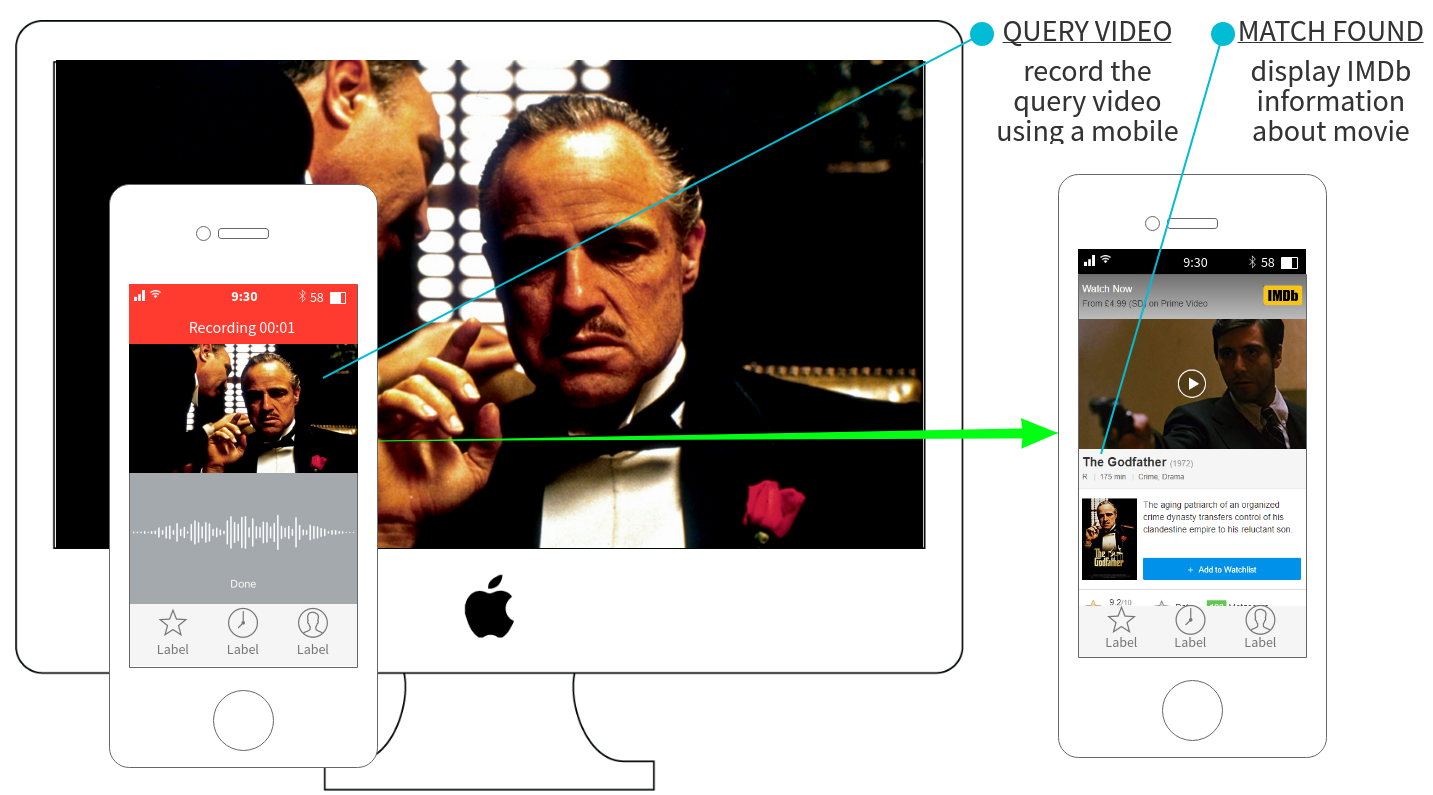
\includegraphics[width=1.15\textwidth]{figures/introduction/system_wireframe.png}}
\caption{\label{fig:wireframe}Wireframe showing the basic high-level concept of an ideal CBVR mobile application for matching movies.}
\end{figure}

%%%%%%%%%%%%%%%%%%%%%%%%%%%%%%%%%%%%%%%%%%%%%%%%%%%%%%%%%%%%%%%%%%%%%%%%%%%%%%%%%%

\section{Report Structure}

\begin{itemize}
    \item \textbf{Introduction}\\
    An overview of the problem description and applications of similar content-based retrieval systems followed by the motivations for this project and the aims to accomplish.
    \item \textbf{Literature \& Technology Survey}\\
    An extensive study of the literature surrounding the topics required to implement the system, including content-based retrieval concepts, visual content extraction and structural video representations.
    \item \textbf{Requirements}\\
    A detailed listing of the different requirements needed to design and implement the system based on the literature survey.
    \item \textbf{Design}\\
    A high-level exploration of potential solutions to meet the previously established requirements and formulate a final solution to implement.
    \item \textbf{Implementation}\\
    A comprehensive examination of the different steps followed to build a system from conception to a functional prototype.
    \item \textbf{Testing \& Evaluation}\\
    A review of the different tests conducted to assess the efficiency of the system and its quality as a whole.
    \item \textbf{Conclusions}\\
    A summary of the accomplished initial project aims, its limitations and plans for future work.
\end{itemize}